\section{Local Indexing} \label{sec:local_indexing}

The local indexing service is responsible for the preprocessing and local storage of intrusion detection datasets. As already described in Section \ref{subsec:clustering}, the data is organized in regions. This means that individual data points are first assigned to a region using a locality-sensitive hash function. Based on the generated hash value, a key is constructed that is used to persist the data point in the respective local pattern database. According to the properties of a locality-sensitive hash function, similar data points are assigned to a common region and thus form a closed processing unit for subsequent operation steps. If a region is formed or an update is made to an existing region, e.g., due to the occurrence of new data, events are emitted to inform the subsequent service. 

\begin{algorithm}
    \caption{Preprocessing and inserting $B \subset D_m$ into $PDB_{L_m}$}
    \label{alg:indexing}
    \algsetup{indent=2em}

    \begin{algorithmic}[1]
        \REQUIRE Pairs of datapoints and labels $B \leftarrow [(\bm{x}_1, y_1), \dots, (\bm{x}_b, y_b)]$
        \ENSURE Regions $R$

        \STATE $R \leftarrow \text{new Set}$
        \FORALL{$(\bm{x}, y)$ in $B$}
            \STATE $\bm{x}' \leftarrow \text{normalize}(\bm{x})$ \COMMENT{see Equation \ref{eq:normalization}}
            \STATE $r \leftarrow h(\bm{x}')$
            \STATE $k_\alpha \leftarrow \text{concatenate}(p_x, r, y)$ \label{alg:indexing_kalpha}
            \STATE $k_\beta \leftarrow g(\bm{x}')$ \label{alg:indexing_kbeta}
            \STATE $k_\gamma \leftarrow \text{concatenate}(p_y,r)$ \label{alg:indexing_kgamma}
            \IF{$PDB_{L_m}[k_\alpha]$ is None}
                \STATE $PDB_{L_m}[k_\alpha] \leftarrow \text{new Hashtable } H$
            \ENDIF
            \IF{$PDB_{L_m}[k_\gamma]$ is None}
                \STATE $PDB_{L_m}[k_\gamma] \leftarrow \text{new Set } S$
            \ENDIF
            \IF{$PDB_{L_m}[k_\alpha][k_\beta]$ is None}
            \STATE $PDB_{L_m}[k_\alpha][k_\beta] \leftarrow (\bm{x}', y)$
            \STATE insert y into Set at $PDB_{L_m}[k_\gamma]$
            \STATE $\text{insert } r \text{ into } R$
            \ENDIF         
        \ENDFOR
        \RETURN $R$
    \end{algorithmic}

\end{algorithm}

First, an intrusion detection dataset $D_m$ is sent to one or more service processors via the $C_{L_m}$. Second, the incoming stream of pairs of data points and labels $(\bm{x}_n, y_n) \in D_m$ is ingested and buffered until a batch $B$ has been accumulated. Then, the batch is preprocessed and inserted into the $PDB_{L_m}$ as described in Algorithm~\ref{alg:indexing}. In words, the datapoint $\bm{x}$ is scaled to the range $[-1, 1]$ by applying a feature-wise min-max normalization, given by

\begin{align}\label{eq:normalization}
    \bm{x}' = \frac{\bm{x}-min(\bm{X}_B)}{max(\bm{X}_B) - min(\bm{X}_B)} \cdot (b - a) + a,
\end{align}

where $a=-1$, $b=1$ and $\bm{X}_B$ is the set of data points within the batch $B$. After that, the scaled data point $\bm{x}'$ is subject to both a locality-sensitive hashing function $h$ and a non-cryptographic hashing function $g$. In this particular architecture, $h$ is a gaussian random projection with a global seed for the initialization of the projection plane $\bm{M}$ (see Section \ref{subsec:random_projection}), such that regions $r = h(\bm{x}')$ across local infrastructures are comparable.

Since the data is organized in regions, a nested scheme is applied for the insertion of pairs of datapoints and labels as depicted in Figure~\ref{fig:indexing}. In fact, the pairs within a region are further partitioned into disjoint subsets according to the label $y$. This means that for each subset of the data of a particular label within a region, a separate hashtable is initialized and inserted into the $PDB_{L_m}$ as a second level. 

Thus, for the persistence of a pair $(\bm{x}', y)$, two keys $k_\alpha, k_\beta \in K$ are constructed (see Lines~\ref{alg:indexing_kalpha}-\ref{alg:indexing_kbeta} in Algorithm~\ref{alg:indexing}). The key $k_\alpha$ is a concatenation of the prefix constant $p_x$, the bit-string $r$ and the label $y$. This way, the data is partitioned primarily by its region and secondarily by its label as described above. The key $k_\beta$ is the result of the non-cryptographic hashing function $g(\bm{x}')$, which serves as a mechanism for deduplicating identical $\bm{x}'$. 

Additionally, a third key $k_\gamma$ is constructed by concatenating the prefix constant $p_y$ and the bit-string $r$. As it is important to retrieve all existing labels within a region efficiently in a processing step of the subsequent service, $k_\gamma$ is used for storing the set of labels within a region as auxiliary metadata.

Next, if not already present, a hash table is initialized and inserted into the slot $PDB_{L_m}[k_\alpha]$. Likewise, if the slot $PDB_{L_m}[k_\gamma]$ is empty, a new set\footnote{A set describes a data structure which is essentially an unordered collection with no duplicate elements.} is initialited and inserted. After that, it is checked if the slot $H[k_\beta]$, which in turn is placed in $PDB_{L_m}[k_\alpha]$, is empty. In the positive case, the pair $(\bm{x}', y)$ is inserted into that slot and the region $r$ is inserted into the set $R$. Otherwise, no data is inserted into the local pattern database and no region is added to $R$. After processing a batch, the set of updated regions $R$ is emitted as events into $C_{L_m}$.

Since data duplicates are filtered before the insert operation in this algorithm, events are also not emitted unnecessarily multiple times if, for example, the same dataset is sent to the service repeatedly. In other words, the inserts are idempotent, which is an important property in this architecture. Since there are operations in subsequent services that are relatively computationally intensive, emitting events is expensive. For this reason, such a streaming application might in practice implement buffers at regular intervals to collect and aggregate the events of several successive batches.



\begin{figure}[t]
    \centering
    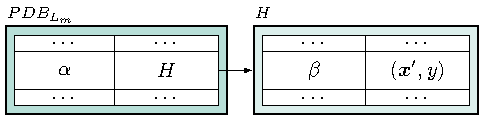
\includegraphics[width=0.8\linewidth]{tikz/indexing.pdf}
    \caption{Nested indexing in a local pattern database.}
    \label{fig:indexing}
\end{figure}

